%
% Quality of Service
%

\section{Quality of service (QoS)}\index{Quantum error correction (QEC)}\index{Quality of service}

\comment{To do}

As discussed previously in Sec.~\ref{sec:QOS}\index{Quality of service}, quality of service is a major consideration in any quantum network. If we are transmitting quantum states over a quantum channel, there will inevitably be deterioration in the form of decoherence, loss, and other undesirable effects we wish to mitigate. In this section we review some of the essential quantum error correction (QEC) techniques that can be used to achieve this.

\comment{Latin quote}\index{Latin}

%
% Entanglement Purification
%

\subsection{Entanglement purification}\index{Entanglement purification}

\comment{To do - move from protocols section. Here do circuit description. Leave optical implementation in protocols section.}

%
% 3-Qubit Code
%

\subsection{3-qubit code}\index{3-qubit code}

\comment{To do}

%
% 9-Qubit Code
%

\subsection{9-qubit code}\index{9-qubit code}

\comment{To do}

%
% Stabiliser Codes
%

\subsection{Stabiliser codes}\index{Stabiliser codes}

\comment{To do}

%
% Surface Codes
%

\subsection{Surface codes}\index{Surface codes}

\comment{These are a particular example of stabiliser codes with an elegant graphical interpretation}

\comment{Missing degree of freedom in stabilisers defines qubit. How does topology (genus) relate to number of logical qubits?}

If the intention is to perform quantum computations using cluster states shared over a network, QEC and fault-tolerance \textit{must} be taken into consideration, or catastrophic algorithmic failure will inevitably follow -- the cluster state model is no different from the circuit model in this respect. Fault-tolerance theory places hard thresholds on the amount of noise (typically depolarising errors and loss) qubits may be subject to in order for fault-tolerance to be possible and computations to succeed. This places strict QoS (Sec.~\ref{sec:QOS}) constraints on the network, which can be accommodated for using the usual depolarising and efficiency cost metrics when developing networking strategies and link performance requirements.

It has been shown that fault-tolerance is possible within the cluster state model \cite{bib:NielsenDawson04, bib:Dawson06} using variations of conventional QEC codes. However, more importantly, from cluster states certain \textit{topological QEC codes} \cite{???} can be readily constructed. This implements a form of QEC-encoded measurement-based quantum computing protocol, where the computation proceeds in a measurement-based fashion, but is `natively' fault-tolerant.

These codes have been shown to have very favourable fault-tolerance thresholds in terms of both depolarising noise and loss \cite{bib:StaceBarrettDohertyLoss, bib:BarrettStaceFT}, as well as frugal resource overhead compared to traditional concatenated codes. Additionally, loss- and gate-failure-tolerant codes, uniquely applicable to the cluster state model, have been described, with very favourable loss thresholds \cite{bib:Varnava05, bib:RalphHayes05, bib:Duan05}. 

Importantly, topological codes do not require joint measurements across the entire graph state, instead requiring only operations localised to small regions within the graph. Thanks to this, computation using such topological codes can remain distributed, without requiring the entire state to be held locally by a particular host, or requiring full access to the entire state by any particular user.

The most common topological code, which we will use here as an example, is the toric code\index{Toric code}, which resides on a lattice graph over the surface of a torus\footnote{As with cluster states, this graph needn't (but could) correspond to a network graph.}. As with cluster states (Sec.~\ref{sec:CSQC}), the toric code is most easily visualised in the stabiliser formalism\index{Stabiliser formalism}. Consider a rectangular sub-graph of the torus. We place a qubit on each edge (not vertex) of the graph. Now we define two sets of stabiliser operators: \textit{star} and \textit{plaquette} operators,
\begin{align} \index{Topological code stabilisers}\index{Star operator}\index{Plaquette operator}
	\hat{S}_\text{star}(v) &= \prod_{i\in e(v)} \hat{X}_i, \nonumber \\
	\hat{S}_\text{plaquette}(p) &= \prod_{i\in e(p)} \hat{Z}_i,
\end{align}
where $e(v)$ are the edges neighbouring vertex $v$, and $e(p)$ are the edges surrounding plaquette $p$. By definition, the toric code state, $\ket\psi_\text{toric}$, satisfies the stabiliser relations,
\begin{align}
	\hat{S}_\text{star}(v) \ket\psi_\text{toric} &= \ket\psi_\text{toric} \,\forall\, v, \nonumber \\
	\hat{S}_\text{plaquette}(p) \ket\psi_\text{toric} &= \ket\psi_\text{toric} \,\forall\, p.
\end{align}
Unlike the cluster state stabilisers from Eq.~(\ref{eq:CS_stab}), these stabilisers are insufficient to fully characterise a unique quantum state. Rather, there are two unspecified degrees of freedom, which allows for a single qubit to be represented. Modifications of the topology, in the form of holes in the lattice (the genus of the topology), allow larger numbers of qubits to be encoded. Logical operations are implemented by performing gates and measurements across topologies over the surface.

The important feature to note is that logical qubits encoded into the toric code do not reside locally at any of the physical qubits in the topology. Rather, they reside jointly across the entire graph, which, like cluster states, might be partitioned across multiple hosts, enabling distributed computation.

This is all summarised in Fig.~\ref{fig:toric_code}.

\begin{figure}[!htb]
	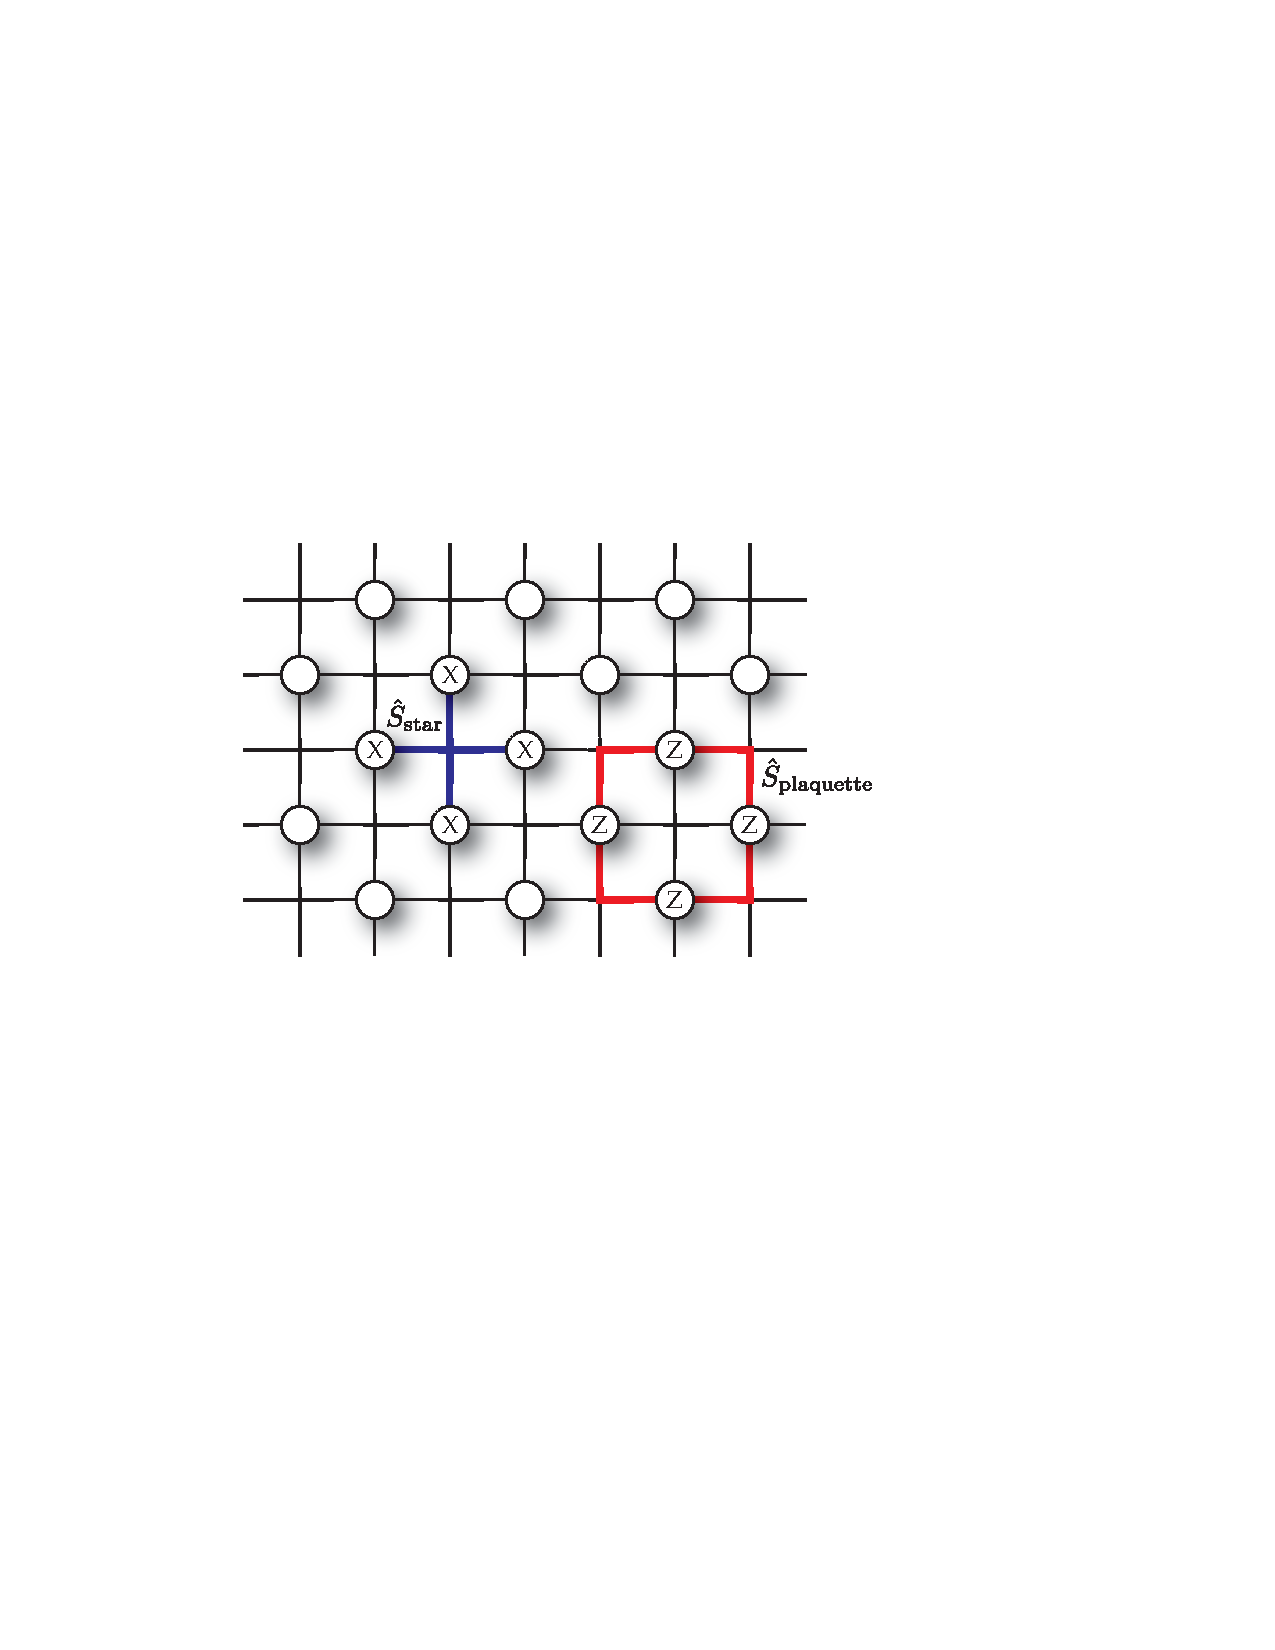
\includegraphics[width=0.47\textwidth]{toric_code}
	\caption{Graph representation of the toric QEC code, and its associated stabilisers. The star and plaquette stabilisers across all vertices, jointly specify the state of the graph up to two missing degrees of freedom, which encode a single logical qubit. Thus, a logical qubit is encoded jointly across the entire graph, not at any specific vertex. Logical operations are performed via operations following topological paths through the lattice (not shown). The graph may be distributed across multiple hosts for distributed quantum computation.} \label{fig:toric_code}
\end{figure}

\comment{How to convert cluster states to topological codes. Add discussion of how to perform gates.}

Having defined the toric code as such, QEC proceeds in a similar manner to any other stabiliser code -- we measure all the stabilisers, yielding a syndrome, from which we can determine geometrically where errors took place in the graph, which can subsequently be corrected (if below threshold).

The simplest example of error detection is the scenario where a single bit-flip ($\hat{X})$ error has occurred in the graph. Now exactly two plaquette stabilisers will yield the $-1$ measurement outcome, instead of the expected $+1$ outcome. These two stabilisers will necessarily be neighbouring ones, overlapping at the qubit where the error took place. Thus, using this geometric property, we are able to identify the location of the single $\hat{X}$ error and subsequently correct it. On the other hand, if there were too many errors, it is possible they could conspire against us to create ambiguity in the geometric argument for the location of the errors. \comment{Figure for both examples of this -- under and over threshold!}

Importantly, the stabilisers are all defined over geometrically localised neighbourhood regions, and do not require long-range measurements, making this type of code suitable to distributed models for quantum computation.

\comment{What about the actual computation? Can this still be distributed when we do the topological gates etc?}

\comment{Figures for thresholds FT and QEC}

%
%
% Topological Codes
%

\subsection{Topological codes} \label{sec:topol_codes} \index{Topological codes}

\comment{Toric code}

%
% Unitary Error Averaging
%

\subsection{Unitary error averaging} \index{Quantum error correction}\index{Unitary error averaging}\label{sec:error_averaging}

\comment{Redundant copies could in principle be distributed}

\comment{To do}

\comment{Add figure}

%
% Gate Failure Codes
%

\subsection{Gate failure codes}\index{Gate failure codes}

\comment{To do}

\comment{Cluster states}

%
% Qubit Loss Codes
%

\subsection{Qubit loss codes}\index{Qubit loss codes}

\comment{cite RohdeHaselgrove}

\comment{Located vs unlocated errors}

\comment{Tree horticultural scheme Rudolph et al.}

%
% Dynamical Decoupling
%

\subsection{Dynamical decoupling}

\comment{To do}

%
% Decoherence-Free Subspaces
%

\subsection{Decoherence-free subspaces}

\comment{To do}

%
% Continuous-Variable Quantum Error Correction
%

\subsection{Continuous-variable quantum error correction}\index{Continuous-variable quantum error correction}

\comment{To do}